\documentclass[10pt]{homework}

\usepackage[utf8]{inputenc}

\usepackage{amsmath}
\usepackage{amssymb}

\usepackage[english]{babel}

\usepackage{blindtext}
\usepackage{minted}
\usepackage{braket}

\usepackage{longtable}

\usepackage{parskip}

\usepackage[open,openlevel=1]{bookmark}
\bookmarksetup{}

\usepackage{fix-unnumbered-sections}


% \usepackage{scrextend}
% \deffootnote{1.5em}{0em}{\textsuperscript\thefootnotemark\,}
% \setlength{\footnotesep}{11pt}

% \hypersetup{
%     colorlinks=true,
%     urlcolor=blue,
% }

\newcommand{\hwauthor}{JAPM}
\newcommand{\hwauthorextra}{}
\newcommand{\hwtitle}{Notes}
\newcommand{\hwshorttitle}{Notes}

% CHANGE THESE ONLY ONCE PER CLASS
\newcommand{\hwclass}{Information Theory}
\newcommand{\hwclassshort}{Information Theory}

\newcommand{\mysep}{\vspace{0.5em} \hrule \vspace{.1in}}
\usepackage{stackrel}

\DeclareMathOperator*{\mysimbig}{\scalebox{2.75}{\raisebox{-0.35ex}{$\sim$}}}
\newcommand{\simover}[1]{
    \overset
        {\resizebox{0.27in}{!}{#1}}
        {\resizebox{0.30in}{!}{$\mysimbig$}}
}

\newcommand{\pluseq}{\mathrel{+}=}
\newcommand{\lelem}[1]{% elementary operations (left alignment)
  \begin{subarray}{l}#1\end{subarray}%
}


\usepackage{bbm}

\usepackage{nicematrix}
\usepackage{tikz}
\usetikzlibrary{fit,shapes.geometric}
\tikzset{highlight/.style={rectangle, draw=black!40, semithick, inner sep=2pt}}

\newcommand{\tikzHlcol}[2]{
    \tikz \node [highlight, fit=(1-#1) (#2-#1)] {} ;
}
\newcommand{\tikzHlrow}[2]{
    \tikz \node [highlight, fit=(#1-1) (#1-#2), inner sep=1pt] {} ;
}

\usepackage{array}   % for \newcolumntype macro
\newcolumntype{M}[1]{>{$\displaystyle\quad}p{#1}<{$}}

\usepackage{mathtools}

\usepackage{bm}

% https://tex.stackexchange.com/questions/343494/
\usepackage{xpatch}
\makeatletter
\AtBeginEnvironment{minted}{\dontdofcolorbox}
\def\dontdofcolorbox{\renewcommand\fcolorbox[4][]{##4}}
\xpatchcmd{\inputminted}{\minted@fvset}{\minted@fvset\dontdofcolorbox}{}{}
\xpatchcmd{\mintinline}{\minted@fvset}{\minted@fvset\dontdofcolorbox}{}{} % see https://tex.stackexchange.com/a/401250/
\makeatother

\newcommand{\indep}{\perp \!\!\! \perp}

\newenvironment{mytable}
    { % begin
        \bgroup
        \centering
        \def\arraystretch{2.3}%  1 is the default, change whatever you need
        \begin{longtable}{wr{0.34\textwidth}M{0.66\textwidth}}
    }
    { % end
        \end{longtable}
        \egroup
    }

\newenvironment{mytextcol}
    { % begin
        \begin{minipage}[t]{0.6\textwidth}
    }
    { % end
        \end{minipage}
    }

% Use for publications...
%\newcommand{\entr}{\mathcal{H}}

\usepackage[overlay,absolute]{textpos}
\newcommand\PlaceText[3]{%
\begin{textblock*}{10in}(#1,#2)  %% change width of box from 10in as you wish
#3
\end{textblock*}
}%

\begin{document}

\PlaceText{0.88\textwidth}{\voffset+1.6cm}{Version: \texttt{\detokenize{2023_06_03_0}}}
\mysetupheader
% TODO: fix this...
% \vspace{1cm}\phantom{M}
%%%%
The author of this document is the sole responsible for all the typos/mistakes found in it and would be grateful to receive corrections and constructive feedback in general.
\\[-20pt]
\section*{References}
\begin{itemize}
    \item
    Stefan Höst, \emph{Information and Communication Theory}, 1st ed., ISBN: 978-1-119-43378-1, Lund University.

% TODO: add McEliece book !!

    \item Raymond W.\@ Yeung, \emph{Information Theory and Network Coding}, 1st ed., ISBN: 978-0-387-79234-7, CUHK.

    \item
    Akshay Krishnamurthy, Aarti Singh, \emph{10-704 Lecture Notes}, Winter 2016-2017, CMU.
    \\
    \url{https://www.cs.cmu.edu/~aarti/Class/10704_Spring15/lecs.html}

    \item
    Eirik Rosnes, \emph{INF 144}, Spring 2017, UiB.
    \\
    \url{https://folk.uib.no/st03333/INF144_2017/Lectures/}

% TODO: http://isl.stanford.edu/~abbas/ee376b/lect02.pdf
    \item
    David Tse, \emph{EE376A Lecture Notes}, Winter 2016-2017, Stanford University.
    \\
    \url{https://tselab.stanford.edu/mirror/ee376a_winter1617/lectures.html}

    \item
    Stefan M. Moser, \emph{IT Lecture Notes}, version 6.9. ETHZ.
    \\
    \url{https://moser-isi.ethz.ch/docs/it_script_v69.pdf}

    % https://www.icg.isy.liu.se/courses/infotheory/

% Robert Gallager
% https://ocw.mit.edu/courses/electrical-engineering-and-computer-science/6-450-principles-of-digital-communications-i-fall-2006/lecture-notes/

% https://ocw.mit.edu/courses/electrical-engineering-and-computer-science/6-451-principles-of-digital-communication-ii-spring-2005/readings-and-lecture-notes/

    \item
    Yury Polyanskiy, Yihong Wu, \emph{Lecture notes on Information Theory}, v.\@\! 2019-May-15, MIT LIDS.
    \\
    Too advanced! (but really good), requires measure theory notions.\\
    \url{http://people.lids.mit.edu/yp/homepage/data/itbook-export.pdf}
\end{itemize}

\section*{Probability}

\subsection*{Basic definitions}

\begin{mytable}

Conditional probability: &
P(A|B) = \frac{P(A \cap B)}{P(B)}
\,;\quad
p_{X|Y}(x|y) = \frac{p_{X,Y}(x,y)}{p_Y(y)}
\\[-8pt]&
\text{given }P(B)\neq 0,\, p_Y(y)\neq 0
\\
Independence ($X \indep Y$): 
& 
p_{XY}(x,y) = p_{X}(x)\cdot p_{Y}(y)
\iff
p_{X|Y}(x|y) = p_{X}(x),\, \forall y\, (\text{with } p(y)\neq 0)
\\

Marginalization (total probability): &
P(X=x) = \sum_{y\in \mathcal Y} P(X=x,Y=y) = \sum_{y\in \mathcal Y} P(Y=y)\cdot P(X=x|Y=y) \\

 &
p_X(x) = \sum_{y\in \mathcal Y} p_{XY}(x,y) = \sum_{y\in \mathcal Y} p_Y(y)\cdot p_{X|Y}(x|y) \\

Expectation: &
\mathbb{E}[X] = \sum_{x\in \mathcal X} x\cdot p_X(x) = \mu_X; \quad
\mathbb{E}[g(X)] = \sum_{x\in \mathcal X} g(x)\cdot p_X(x)
\\

Variance: &
\mathbb{V}[X] = \mathbb{E} [(X-\mu_X)^2] = \sigma_X^2 \text{, where } \mu_X = \mathbb{E}[X]\\
Power (Mean Square): & \mathbb{E}[X^2] = \mathbb{V}[X]  + (\mathbb{E}[X])^2
\\

Covariance: &
\text{Cov}(X,Y) = \mathbb{E}_{XY} [(X-\mu_X)\cdot (Y-\mu_Y)] = \mathbb{E}_{XY} [X\cdot Y] -\mu_X \cdot \mu_Y
\\

RV linear combination: &
Y = \sum_{i=1}^{N}\alpha_n\cdot X_i \implies
\mathbb{E}[Y]=\sum_{i=1}^{N}\alpha_i\cdot \mathbb{E}[X_i]
\\ &
\mathbb{V}[Y] = \sum_{i=1}^{N}\alpha_n^2\cdot \mathbb{V}[X_n] 
+ 2\cdot \sum_{i=1}^{N}\sum_{j=i+1}^{N} \text{Cov}(X_i, X_j)
\\

Entropy (discrete RV): &
H(X) = \mathbb{E}_X[-\log_2(p_X(X))]\text{ bits};
\quad H_e(X) = \ln 2\cdot H(X)\text{ ``nats''}
\\[-8pt]
& H(X) = H(p_1, p_2, \cdots, p_n) = \sum_i p_i\cdot \log \frac{1}{p_i}
\\

Differential entropy (continuous RV): &
H_\text{Dif}(X) = \mathbb{E}_X[-\log_2(f_X(X))] = \int_{\mathbb{R}} f_X(x)\cdot\log_2 \frac{1}{f_X(x)}\, dx, \newline\phantom{M} (X \text{ with pdf } f_X)
\\\pagebreak

Wide-Sense Stationary (WSS) process: &
E[X_i] = E[X_1]; \quad r_{XX}(n, n+k) = r_{XX}(k)
\\
(Strongly/Strictly) Stationary process: &
p_X(x_{1},x_{2}, \cdots ,x_{n}) = 
p_X(x_{1+\Delta},x_{2+\Delta}, \cdots ,x_{n+\Delta}) 
\newline\phantom{M}
\text{(time shift invariance)}
\\

Ergodic process: &\text{WSS and (in mean) }
\hat\mu_X = \langle X_i \rangle_N = \frac{1}{N}\sum^N{X_i} = \mathbb{E}[X_0] = \mu_X\\
% &\text{(in autocovariance) }\newline\phantom{MM} \hat r_{XX}(\tau) = (????) = \mathbb{E}[(X_t-\mu_{X_t})(X_{t-\tau}-\mu_{X_{t-\tau}})] = r_{XX}(\tau)
% \\
\end{mytable}

\subsection*{Basic properties}

\begin{mytable}
Bayes' theorem: &
p_{X|Y}(x|y) =
\frac{p_{Y|X}(y|x)\cdot p_X(x)}{p_Y(y)} =
\frac{p_{Y|X}(y|x)\cdot p_X(x)}{
    \sum\limits_{x^\prime\in\mathcal{X}} p_{Y|X}(y|x^\prime)\cdot p_X(x^\prime)
}
\\

Chain rule: &
P(X_1,X_2, \dots, X_n) = P(X_1,X_2, \dots, X_{n-1})
\cdot P(X_n|X_1, X_2, \dots, X_{n-1})
\\
 &
= \cdots =
\overbrace{\underbrace{P(X_1)\cdot P(X_2|X_1)}_{P(X_1,X_2)}
\cdot P(X_3|X_1,X_2)}^{P(X_1,X_2,X_3)} \cdots 
 P(X_n|X_1, X_2, \dots, X_{n-1})
\\[-4pt]
 &
= \prod_{i=1}^n P(X_i | X_1, X_2, \dots, X_{i-1}), \quad \text{(convention: first factor is $P(X_1)$)}
\\

Markov's inequality: &
P(X>a) \le \frac{\mathbb{E}[X]}{a}
\quad \text{($X$ is a nonnegative RV)}
\\
Chebyshev's inequality: &
P\left(\left|X-\mathbb{E}[X]\right|>\varepsilon\right) \le \frac{\mathbb{V}[X]}{\varepsilon^2};
\quad 
P\left(\left|X-\mathbb{E}[X]\right|>\frac{\sigma_X}{\varepsilon}\right) \le \varepsilon^2
\\
Weak Law of Large Numbers (LLN): & Y_N = \frac{1}{N}\sum_{i=1}^{N} X_i \quad (X_i \text{ i.i.d.});
\quad 
P\left(\left|Y_N-\mathbb{E}[X]\right|>\varepsilon\right) \le \frac{\mathbb{V}[X]}{\varepsilon^2}
\\&
\lim_{N\to\infty} P\left(\left|Y_N-\mathbb{E}[X]\right|<\varepsilon\right) = 1; 
\quad
Y_N \xrightarrow[]{P} \mathbb{E}[X] 
\\
%Convergence in probability:
%& \text{[TODO]}
%\\
Central Limit Theorem (CLT): & Y_N = \frac{1}{N}\sum_{i=1}^{N} X_i \quad (X_i \text{ i.i.d., } \mathbb{E}[X_i] = \mu,\,\mathbb{V}[X_i]=\sigma^2)
\\&
\frac{Y_N-\mu}{\sigma/\sqrt{N}}
\,\simover{$(N\to\infty)$}\,
\mathcal{N}(0,1) 
\\
Convexity:&
f(\lambda \cdot x_1+(1-\lambda) \cdot x_2) \le 
    \lambda\cdot f( x_1 ) + (1-\lambda)\cdot f( x_2 ),\, \forall\lambda \in [0,1]
\\
Concavity:& \text{$f$ is convex $\iff$ $-f$ is concave}
\\

Jensen's inequality: & g \text{ is convex} \implies \mathbb{E}[g(X)] \ge g(\mathbb{E}[X])
\\

Log-sum inequality: & \sum_i a_i \cdot \log \frac{a_i}{b_i} \ge
A \cdot \log \frac{A}{B}; \quad A =\sum_i a_i; \, B =\sum_i b_i; \, a_i > 0,\,b_i > 0
\\

IT inequality: & \log_B (r) \le (r-1)\cdot \log_B(e); \\[-10pt]&
\text{``$\log x$ is concave so it lies below its tangent line at $(1,0)$''}
\\

\end{mytable}

\newpage
\subsection*{Discrete Distributions}

Hint -- Use combinatorics: \url{https://en.wikipedia.org/wiki/Urn_problem}

\begin{mytable}

Uniform (discrete):  & X\sim U(n),\quad
p_X(x) = \frac{1}{|\mathcal{A}|}\cdot \mathbbm{1}_\mathcal{A}(x),\quad \mathcal{A} = \{0,\dots, n-1\} \subset \mathbb{N}, \, |\mathcal{A}| = n 
\\
& \mathbb{E}[X] = \frac{n-1}{2}; \quad \mathbb{V}[X] = \frac{n^2-1}{2};
\quad H(X) = H(p, p, \dots, p) = \log_2 p
\\

Bernoulli:&\text{``heads or tails (loaded coin), black/white ball, success/failure, 1 or 0, ...''}
\\[-8pt]
&
X\sim\text{Be}(p); \quad
P(X=\text{``1''}) = p = 1 - P(X=\text{``0''}) 
\\[-12pt]
& \mathbb{E}[X] = p; \quad \mathbb{V}[X] = p\cdot (1-p);
\quad H(X) = h_2(p) = H(p, 1-p)
\\[-6pt]
&\begin{mytextcol}
``Probability of $k$ successes (with prob.\,$p$) in $n$ attempts'' = \\= ``Probability of a binary string of length $n$ with $k$ ones'' =\\ = $P(\bm X=\bm x)=p^k\cdot (1-p)^{n-k}$
\end{mytextcol}
\\
Geometric: & 
\text{``infinite attempts where the first success is at the }k\text{-th attempt''}
\\ & 
X\sim\text{Ge}(p),
\quad p=P(X=\text{``}\underbrace{\text{00...01}}_k\text{...''})
\\
&
p_X(k)= p\cdot (1-p)^{k-1};
\quad
\mathbb{E}[X] = \frac{1}{p}; \quad \mathbb{V}[X] = \frac{1-p}{p^2}; \quad H(X) = \frac{h_2(p)}{p}
\\
Binomial:
&
\text{``number of ones (successes) out of }n\text{ attempts (with replacement)''}
\\&
X\sim \text{Bin}(n,p),
\quad p=P(X_{\text{Bern}(i)}=\text{``1''})
\\&
p_X(k) = \binom{n}{k}\cdot p^k\cdot (1-p)^{n-k}
\\&
\mathbb{E}[X] =n\cdot p ; \quad \mathbb{V}[X] = n\cdot p\cdot (1-p); \\& H(X) = \frac{1}{2}\cdot \log_2\left(2\pi \cdot e\cdot n\cdot p\cdot (1-p)\right) + \mathcal{O}(1/n)
\\

Hypergeometric:
&
\begin{mytextcol}
``number of black balls (successes) out of $n$ total balls drawn \emph{without replacement} from an urn with initially $N$ balls, of which $K$ are black''.
\end{mytextcol}
%
\\&
X\sim \text{Hypergeometric}(N,K,n);\quad \left(n=1\implies X\sim Be(p), \, p=K/N\right)
\\&
p_X(k) = \frac{\binom{K}{k}\binom{N-K}{n-k}}{\binom{N}{n}}
;\quad \mathbb{E}[X] =n\cdot \frac{K}{N}
\\&
\begin{mytextcol}
\footnotesize{Sometimes `hypergeometric' refers to the multivariate hypergeometric distribution (multiple colors), here we refer only to the \emph{bivariate} distribution (2 colors: black and white). Also, this is different from the  `multinomial distribution' which is the `with replacement' case, the generalization of the binomial distribution.}
\end{mytextcol}
\end{mytable}

%\pagebreak
\subsection*{Continuous Distributions}
\begin{mytable}
Uniform (continuous):  & X\sim U(a, b),\quad
f_X(x) = \frac{1}{\Delta}\cdot \mathbbm{1}_\mathcal{A}(x),\quad \mathcal{A} = [a, b] \subset \mathbb{R}, \, \Delta = b - a
\\
& \mathbb{E}[X] = \frac{a+b}{2}; \quad \mathbb{V}[X] = \frac{\Delta^2}{12}; \quad H_\text{Dif}(X) = \log_2 \Delta
\\

Gaussian distribution: & X \sim \mathcal N(\mu, \sigma), \,\sigma > 0
\\
& f_X(x)=\frac{1}{\sqrt{2\pi\sigma^2}}\cdot
\exp\left[-\frac{1}{2}\left(\frac{x-\mu}{\sigma}\right)^2\right]
\\
& \mathbb{E}[X] = \mu; \quad \mathbb{V}[X] = \sigma^2; \quad H_\text{Dif}(X) =
\frac{1}{2}
\log_2(2\pi\cdot e\cdot \sigma^2)
\\

Exponential distribution: & X \sim \text{Exp}(\lambda), \,\lambda > 0 \implies
f_X(x) = \lambda \cdot e ^ {-\lambda x}, \, x\ge 0
\\
& \mathbb{E}[X] = \frac{1}{\lambda}; \quad \mathbb{V}[X] = \frac{1}{\lambda^2}
\\
\end{mytable}

\newpage
\section*{Information and entropy}

\begin{mytable}
Hartley's information measure: & I_H(X) = \log k = \log |\mathcal{X}|
\\[-8pt]&
\text{Number of possible outcomes (disregarding probabilities).}
\\[-8pt]&
I_H(X_1,X_2, \cdots, X_n) = \log k^n = n\cdot I_H(X)
\\
Mutual information (between events):
& I(A;B) = \log \frac{P(A|B)}{P(A)} = \log \frac{P(A\cap B)}{P(A)\cdot P(B)} = I(B;A)
\\
Bounds on $I(A;B)$:
&
-\infty \le I(A;B) \le \min \{
    -\log P(A), \, -\log P(B)
\}
\\&
\begin{cases}
    P(A|B) = 0 \implies
    ( B \Rightarrow \lnot A ) \implies
    A \cap B = \varnothing \implies
    I(A;B) = -\infty
\\
    P(A|B) = 1 \implies
    ( B \Rightarrow A ) \implies
    A \subseteq B \implies
    I(A;B) = -\log P(A)
\\
    P(B|A) = 1 \implies
    ( A \Rightarrow B ) \implies
    B \subseteq A \implies
    I(A;B) = -\log P(B)
\\
    P(A|B) = P(A) \implies
    A \indep B \implies  I(A;B) = 0
\end{cases}
\\
Self-information (of an event):&
I(A) = I(A;A) = -\log P(A) \ge 0
\\
Entropy (of a discrete RV):&
H(X) = \mathbb{E}_x[I(X=x)]  = \mathbb{E}_X[-\log p_X(X)] = -\sum_x p_X(x)\cdot \log p_X(x)
\\[-12pt]&
H(X)\ge 0
\\[-8pt]&
\text{Notation: }H(p_1, p_2, \cdots, p_n) = -\sum_i p_i\cdot \log p_i, \,\,\, \text{ given } \sum_i p_i = 1, p_i\ge 0
\\
Binary entropy function:
& h_2(p) = H(p, 1-p),\, 0\le p\le 1;  \, \quad \frac{\partial h_2(p)}{\partial p} = \log_2 \frac{1-p}{p} = -\mathrm{logit}_2\,p 
\\
Entropy bounds:& 0 \le H(X) \le \log k, \,\, k = |\mathcal{X}|
\\&
H(X)=0 \Rightarrow X\text{ deterministic};\,H(X)=\log k \Rightarrow X\sim\text{Uniform}(k)
\\&
H(X) \le \log k = I_H(X=x) = H\left(\frac{1}{k}, \frac{1}{k}, \cdots, \frac{1}{k}\right)
\\
Property for 3 outcomes:
&H(p_1,p_2,p_3) = h(p_1) + (1-p_1)\cdot h\left(\frac{p_2}{1-p_1}\right), \text{ given }p_1\neq 1
\\
Property for $N$ outcomes:
&H(p_1,p_2,\cdots,p_N) = h(p_1) + (1-p_1)\cdot H\left(\frac{p_2}{1-p_1},\frac{p_3}{1-p_1},\cdots \frac{p_N}{1-p_1} \right) \newline\phantom{M}\text{given }p_1\neq 1
\\
Permutation invariance:
&
\begin{mytextcol}
$H(X) = H(f(X))$, for $f$ injective (usually bijective, i.e.~invertible)\\ (a.k.a.\@ invariance under relabeling)\\[5pt]
In general: $H(X) \ge H(f(X))$
\end{mytextcol}
\\
Joint entropy: &
H(X,Y) = \mathbb{E}_{XY}[-\log p(X,Y)]  = -\sum_x \sum_y p_{XY}(x,y)\cdot \log p_{XY}(x,y)
\\[-8pt] &
H(X_1,X_2, \cdots, X_n) = \mathbb{E}_{\bm X}[-\log p(\bm X)] 
\\
Entropy conditioned on an outcome: &
H(X|Y=y) = H(X|\{Y=y\}) = - \sum_x p_{X|Y}(x|y) \cdot \log p_{X|Y}(x|y) \\
Conditional entropy: &
H(X|Y) = \mathbb{E}_y[H(X|\{Y=y\})] = \sum_y H(X|\{Y=y\}) \cdot p_Y(y)
\\&
H(X|Y) = \mathbb{E}_{XY}[-\log p(X,Y)]  = -\sum_x \sum_y \underbrace{p_{XY}(x,y)}_\text{!!!}\cdot \log p_{X|Y}(x|y)
\\\pagebreak
Mutual information (between RVs):
& I(X;Y) =  \mathbb{E}_{XY}[I(X=x;Y=y)] = I(Y;X)
\\ &
I(X;Y) = H(X) - H(X|Y) = H(X) + H(Y) - H(X,Y)
\\&
\phantom{MM}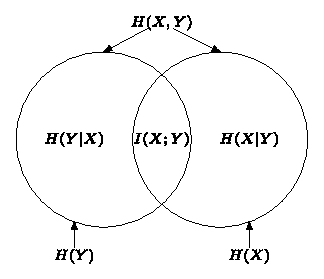
\includegraphics[width=0.3\textwidth]{img_Polyanskiy_mutual.pdf} \text{\footnotesize{(source: Y.\@ Polyanskiy IT\,lectures)}}
\\ &
I(X;Y) =\mathbb{E}_{XY}\hspace{-1.4mm}\left[\log \frac{p_{XY}(x,y)}{p_X(x)\cdot p_Y(y)}\right] = \sum_{x,y}p_{XY}(x,y)\cdot \log\frac{p_{XY}(x,y)}{p_X(x)\cdot p_Y(y)}
\\
Conditioning reduces entropy: &
I(X;Y) = H(X) - H(X|Y) \ge 0 \Rightarrow H(X) \ge H(X|Y) \text{, equal iff }X\indep Y
\\
RV self-information is entropy: &
H(X|X) = 0 \implies I(X;X) = H(X)
\\
Mutual info.\,is bounded by entropy:
& H(X) \ge H(X) - H(X|Y) = I(X;Y)
\\[-8pt]&\phantom{M}
\implies I(X;Y) \le \min\{H(X),H(Y)\}
\\[-8pt]&
\text{Also: } \max_{p_X(x)} H(X) = \log |\mathcal X| = I_H(X) \\[-8pt]&\phantom{M}
\implies
I(X;Y) \le \min\{\log |\mathcal X|,\log |\mathcal Y|\} 
\\
Conditional mutual information: &
I(X;Y|Z) =
\mathbb{E}_{XYZ}\left[\log
    \frac{p(X,Y|Z)}{p(X|Z)p(Y|Z)}
\right] =
\sum_{x,y,z} p(x,y,z)\log
    \frac{p(x,y|z)}{p(x|z)p(y|z)}
\\&
I(X;Y|Z) =
    H(X|Z)+H(X|Z)-H(X,Y|Z)
\\&
I(X;Y|Z) =
    H(X|Z)-H(X|Y,Z)=H(Y|Z)-H(Y|X,Z)
\\
Chain rule for entropy: &
H(X,Y) = H(X|Y) + H(Y) = H(Y|X) + H(X) \le H(X) + H(Y)
\\&
H(X_1, X_2, \cdots, X_n) = \sum_{i=1}^n H(X_i|X_1,X_2,\cdots X_{i-1}) \le \sum_{i=1}^n H(X_i)
\\
KL divergence (a.k.a.\,relative entropy):
&
D(p||q) = \mathbb{E}_p\left[\log\frac{p(X)}{q(X)}\right] =
\sum_x p(x) \cdot \log\frac{p(x)}{q(x)} \ge 0
\\&
\text{in general:}
\begin{cases}
\text{no symmetry,}&
    D(p||q) \neq D(q||p)\\
\text{no triangle inequality,}&
D(p||q) + D(q||r) \ngeq D(p||r)
\end{cases}
\\
Mutual information as KL div.:
&
I(X;Y) = D(p_{XY}(x,y)||p_X(x)\cdot p_Y(y)) \ge 0
\\
Entropy rate (of a random process): &
H_\infty(X) = \lim_{n\to\infty}\frac{1}{n}\cdot H(X_1,X_2,\cdots,X_n)
\\
\emph{Alternative} entropy rate: &
H(X|X^\infty) = \lim_{n\to\infty} H(X_n|X_1,X_2,\cdots,X_{n-1})
\\[-12pt]
&\text{Equality in stationary processes: } H_\infty(X) = H(X|X^\infty)
\\
Bounds for stationary processes: &
0\le H_\infty (X)\le H(X) \le \log k; \quad H(X) = H(X_i)
\end{mytable}

\section*{Markov chains}

\begin{mytable}

Markov property: &
P(X_i | X_{i-1}, \cdots, X_1) = P(X_i|X_{i-1}),\,\,\forall i>1\\
&\text{The RVs } X_i\text{ are in a total order (\emph{chain}): } X_1\to X_2 \to \cdots \to X_N
\\
Time-invariant (TI) Markov chains: &
p(x_i|x_{i-1}) = p(x_{i+\ell}|x_{i-1+\ell}) \text{ (assumed in general)}
\\
Chain rule for Markov chains: &
P(X_1,X_2, \dots, X_N) = \prod_{i=1}^n P(X_i | X_1, X_2, \dots, X_{i-1}) =
\\
 &
= P(X_1)\cdot \prod_{i=2}^N P(X_i | X_{i-1}) 
\stackrel{\text{(TI)}}{=}
 P(X_1)\cdot  \left( P(X_2 | X_{1})\right)^{N-1}
\\
 &
H(X_1,X_2,\cdots,X_N) =
    H(X_1) + \sum_{i=2}^{N} H(X_i|X_{i-1})
\newline\phantom{MMMMMMMM...}
\stackrel{\text{(TI)}}{=}
H(X_1) + (N-1)\cdot H(X_2|X_{1})
\\
State transition matrix:&
\mathcal P = [p_{ij}]; \quad p_{ij} = p_{X_2|X_1}(x_i|x_j), \quad i\text{-th row adds up to }1
\\[-6pt]&
\pi_k^{(n)} = P(X_n=x_k),
\quad \bm{\pi}^{(n+1)} = \bm{\pi}^{(n)}\cdot \mathcal P
\quad \text{($\bm \pi^{(n)}$ are row vectors)}
\\

Asymptotic distribution:&
\bm{\pi} = \lim_{n\to \infty} \bm{\pi}^{(n)} = \lim_{n\to \infty} \bm{\pi}^{(0)} \cdot \mathcal P^n; \quad \lim_{n\to \infty} \mathcal P^n =
\bgroup\def\arraystretch{1}
\begin{pmatrix}
    \bm{\pi} \\
    \vdots \\
    \bm{\pi} \\
\end{pmatrix}\egroup ; \quad \bm\pi\cdot \mathcal P = \bm\pi
\\
Existence (and uniqueness) of $\bm\pi$:
& \exists n_0 >0 \text{ s.t.\,all entries of } \mathcal P^{n_0} \text{ are strictly positive (nonzero)} \implies \exists!\bm \pi
\\[-12pt] &
\text{(particular case of Perron–Frobenius thrm.\@ for strongly connected graphs)}
\\

Computation of $\bm\pi$:
&
\begin{cases}
    \bm\pi \cdot (\mathcal P-I) = 0 & \text{ (rank $N-1$ due to $\mathcal P$'s nullspace dimesnion)} \\
    \sum_k \pi_k = 1 & \text{ (extra equation needed for full rank)}
\end{cases}
\\
$H_\infty(X)$ of a stationary Markov chain: &
H_\infty(X) = H(X_2|X_1)=
\\[-12pt]&
H_\infty(X) = \sum_i \bm\pi_i\cdot H(X_2|X_1=x_i); \quad
H(X_2|X_1=x_i)=-\sum_j p_{ij}\log p_{ij}
\\[-12pt]&
H_\infty(X)\text{ is the min.\,average info required to encode one transition.}
\\
Data processing lemma:
& X\to Y\to Z \text{ is a Markov chain} \implies
\begin{cases}
    I(X;Z) \le I(X;Y) \\
    I(X;Z) \le I(Y;Z)
\end{cases}
\\
&
I(X; Z) = H(X) - H(X|Z) \le H(X) - H(X|YZ) =\newline\phantom{MMMMMMMMMMM.M}= H(X) - H(X|Y) = I(X;Y)  
\end{mytable}
\section*{Source coding}

\begin{mytable}
Compression ratio: & R = \frac{\#\text{Source bits}}{\#\text{Compressed bits}}, \quad \text{($R > 1$, except in pathological cases)}
\\
Classification of source codes: &
\begin{mytextcol}
\begin{itemize}
    \item Non-singular codes: coding is injective (lossless compression)
    
    $\bm x_1 \neq \bm x_2 \implies C(\bm x_1) \neq C(\bm x_2)$
    \item Uniquely decodable codes: sequence of symbols is unambiguously decodable (\emph{extension} code is non-singular)
    
    Sequences $\bm x_1^n \neq \bm x_2^m \implies C_{ext}(\bm x_1^n) \neq C_{ext}(\bm x_2^m)$
    
    where $C_{ext}(\bm x^n) = \text{Concat}(C(\bm x_{(1)}),...,C(\bm x_{(n)}))$
    \item Prefix codes: no codeword is prefix of any other codeword.
\end{itemize}
\end{mytextcol}
\\
Average codeword length: &
L=\mathbb{E}[\ell_x] = \sum_x p_X(x)\cdot\ell_x
\\
Path length lemma: &
L=\sum_{n_i\in\text{\,``inner nodes''}} p(n_i)
\quad \text{ (valid for prefix codes)}
\\
Kraft inequality: &
\sum_{i=1}^k D^{-\ell_i}\le 1 \text{ (valid for }D\text{-ary prefix codes)}
\\[-4pt] &
\text{all prefix codes must obey this constraint.}
\\
McMillan inequality: &
\begin{mytextcol}
Kraft inequality also holds for $D$-ary uniquely decodable codes.\\
Therefore, those are also subject to the same constraint.
\end{mytextcol}
\\
$L$, lower bound: &
L \ge H_D(X) = \frac{H(X)}{\log_2 D}
\\ & \text{equality if all }\ell_x =-\log_D p(x)
\text{ (only possible if all are integers)}
\\
$L$, achievable upper bound: &
    L < H_D(X)+1 \text{ (for some }D\text{-ary prefix code, guaranteed to exist)}
\\
Shannon-Fano code &
\begin{mytextcol}
Prefix code with $\displaystyle\ell_{x_i} = \lceil -\log_D p(x_i) \rceil $
\\[8pt]
$L$ below upper bound, may have unused leaves, not optimal in general
\end{mytextcol}
\\
Fano code: &
\begin{mytextcol}
  ``Binary partition into sets as equiprobable as possible''.\\[3pt]
  $L$ is similar to Shannon-Fano code.\\[3pt]
  Provided sorted probabilities: $ p_1\ge p_2\ge\cdots\ge p_k$, \\[3pt]
  recursively split at index $q$ that minimizes:
    $\displaystyle
    \left|\sum_{i=1}^q p_i - \sum_{i=q+1}^k p_i\right|
    $
\end{mytextcol}
\\

Huffman code: &
\begin{mytextcol}
Tree algorithm: replace smallest (least prob.)\@ 2 nodes with an inner node with their sum; repeat until only one node (root) remains.\\[3pt]
Optimal: no better binary prefix code in terms of $L$.

Note: [verify this claim??] if an optimal code is built using a distribution $q(x)$, but it is applied to a source with a distribution $p(x)$, then the resulting average codeword length is equal to the cross-entropy (used in MachLearn field): $L = \mathbb{E}_p[q] = - \sum p(x) \log q(x)$
\end{mytextcol}
\\

Optimal code for i.i.d.\,sequences: &
\bm{X} = (X_1,\cdots,X_n); \quad \bm{x} \xmapsto[]{\text{Huff}_n}
\bm{y}; \quad |\bm{y}| = \ell^{(n)}_{\bm{x}}; \quad L^{(n)} = \mathbb{E}[\ell^{(n)}_{\bm{x}}]
\\&
H(X_1,\cdots X_n) \le L^{(n)} \le H(X_1,\cdots X_n) + 1
\\&
\xRightarrow[]{\text{i.i.d}}
n\cdot H(X_1) \le L^{(n)} \le n\cdot H(X_1) + 1; \quad H(X) = H(X_1)
\\
Optimal $L$ for i.i.d.\,sequences: &
H(X) \le L \le  H(X) + \frac{1}{n}
;\quad
\left[L=
\frac{\mathbb E[\ell_{\bm x}]}{n}=\frac{L^{(n)}}{n}\right]
\\&
\lim_{n\to \infty} L = H(X) \quad \text{(length per symbol $L$ is optimized as $n$ increases)}
\\
Optimal $L$ for ergodic processes: &
H(X_1,\cdots X_n) \le L^{(n)} \le H(X_1,\cdots X_n) + 1
\\&
\implies \frac{1}{n}\cdot H(X_1,\cdots X_n) \le L \le \frac{1}{n} \cdot H(X_1,\cdots X_n) + \frac{1}{n}
\\&
\implies \boxed{\lim_{n\to \infty} L = H_\infty(X)} \le H(X) = H(X_1) \\[-6pt]
&\begin{mytextcol}
Better than i.i.d.\\(cannot be attained by Huffman codes unless symbols are grouped)
\end{mytextcol}
\\\end{mytable}

\newpage
\section*{Universal compression/source coding}
A source code is universal if it can be constructed without knowledge of the statistics of the
source.
\begin{mytable}
LZ77 codeword: &
\bm y = (j,l,c); \text{ where:}\begin{cases}
    j,&\text{match offset (in $S$, from the right)}\\
    l,&\text{match length (can overlap $B$)}\\
    c,&\text{character after the match (in $B$)}
\end{cases}
\\&
\begin{cases}
\text{no match }&\implies j=0,\, l=0,\, c=\text{``first char in $B$''}
\\
\text{match }&\implies j>0,\, l>0
\end{cases}
\\[-4pt]&
\text{If match, advance buffers 
$l+1$
chars (otherwise: $1$ char)}
\\[-4pt]
LZ77 codeword length: &
\ell_{\bm y} = \ell((j,l,c)) = 
\lceil \log(S+1) \rceil +
\lceil \log(B+1) \rceil +
|c|
\\[-8pt]
& |c| = \lceil \log k \rceil \text{; when }c\in \text{``ASCII 8-bit'', }|c| = \log_2 2^8 =8 \text{ bits}
\\
LZ77 total compressed size: &
 \underbrace{S \cdot |c|}_\text{initial buffer} + \sum_i \ell_{\bm{y}_i} = {S \cdot |c|} + N_{cw} \cdot \ell_{\bm{y}}, \quad N_{cw} = \text{num.\,of codewords}
\\
LZSS codeword: &
\bm y = \begin{cases}
    (0,j,l),&\text{match}\\
    (1, c),&\text{no match}\\
\end{cases}
; \text{ where:}\begin{cases}
    j,&\text{match offset (never $0$)}\\
    l,&\text{match length (never $0$)}\\
    c,&\text{first char in $B$}
\end{cases}
\\[-4pt]&
\text{If match, advance buffers $l$ chars (otherwise: $1$ char)}
\\
LZSS codeword length: & \ell_{\bm{y}} = 
\begin{cases}
    \text{match:} &
    1 + \lceil \log(S+1) \rceil +
    \lceil \log(B+1) \rceil
    \\
    \text{no match:} &
    1 + |c|
\end{cases}
\\
LZSS total compressed size: &
 \underbrace{S \cdot |c|}_\text{initial buffer} + \sum_i \ell_{\bm{y}_i} =
  S \cdot |c| +
  N_\text{match} \cdot \ell_{\text{match}} +
  N_\text{no-match} \cdot \ell_{\text{no-match}}
\\
LZ78: & [...] \text{Dictionary} [...]
\\
LZW: & [...] \text{Dictionary with preinitialization (usually with the 1-char entries)} [...]
\end{mytable}

\newpage
\section*{Asymptotic Equipartition Property or Principle (AEP)}
\begin{mytable}
AEP concept: &
\begin{mytextcol}
  There exists some class/set of sequences $A_\varepsilon^{(n)}$ of length $n$ called \emph{typical} such that, as $n$ increases ($n\to\infty$), they become almost sure ($P\to 1$), and, at the same time, they remain a negligible portion (as $\varepsilon\to 0$) of the total set of sequences of length $n$, $\mathcal X^{(n)}$, with the only exception of the sequence generated by the uniform distribution with support $\mathcal X$.\\
  Incidentally, sequences that are individually the most probable tend not to be in $A_\varepsilon^{(n)}$, i.e. are \emph{atypical} (same for the \emph{least} probable ones).
  \\
  The typical sequences are defined as precisely those that enable the convergence to $H(X)$ using Weak LLN (i.e.\@ convergence in probability).

% TODO: It also happens that those sequences tend to not contain
%       the most probable words nor the least probable words.
%       (see Sergio Verdú video).
\end{mytextcol}
\\
Sequence of $n$ i.i.d.\@ RVs: &
\begin{mytextcol}
``$\bm X$ is i.i.d'' means the sequence of $n$ RVs $\bm X = (X_1, X_2, \cdots, X_i, \cdots, X_n)$\\ with $\bm X \in \mathcal{X}^n$ has the property: $X_{i}, X_{j}$ are i.i.d., $\forall i,j; i \neq j$\\ (i.e.\@ pairwise i.i.d.)
\end{mytextcol}
\\
Set of $\varepsilon$-typical sequences for i.i.d.\@ RVs: &
\text{Given a sequence $\bm X$ of $n$ i.i.d.\@ $n$ RVs, for each and $\varepsilon>0$ define:}
\\[-8pt]&
A_\varepsilon^{(n)} (X) = \left\{
    \bm x = (x_1,x_2,\cdots,x_n):
\,
\left|
-\frac{1}{n}\log p_{\bm X}(\bm x)-H(X)
\right|\le \varepsilon
\right\} =
\\&
A_\varepsilon^{(n)} (X) = \left\{
    \bm x = (x_1,\cdots,x_n):
\,
2^{-n\cdot(H(X)+\varepsilon)}
\le p_{\bm{X}}(\bm x)
\le
2^{-n\cdot(H(X)-\varepsilon)}
\right\}
\\
AEP (Weak LLN redux): &
\text{Because $\bm X$ are i.i.d.:}\, -\frac{1}{n}\log p_{\bm X}(\bm X) =
-\frac{1}{n}\log \prod_{i} p_{X}(X_i) \stackrel[n\to\infty]{P}{\longrightarrow} H(X)
\\&
\forall\varepsilon>0,\, \exists n_0:\, \forall n>n_0 \implies
P(``\bm x \in A_\varepsilon^{(n)} (X) ") \ge 1-\varepsilon
\\&
\text{Main idea: } \underset{(n,\,\varepsilon)\to(\infty,\,0^+)}{\text{lim}^*}\, P(``\bm x \in A_\varepsilon^{(n)} (X) ") = 1
\\[-0.3cm]&\text{\footnotesize{${}^*$Note: this is not actually a limit...}}
\\[-0.3cm]&
\begin{mytextcol}
Also we have (as $\varepsilon\to 0$): $p_{\bm X}(\bm x)|_{\bm x\in A_\varepsilon^{(n)}} 
\approx 2^{-n H(X)};\quad p_{\bm X}(\bm x)|_{\bm x\notin A_\varepsilon^{(n)}} \approx 0$
\\ (i.e.\@ sequences inside the typical set tend to be equiprobable and sequences outside of it tend to be impossible)
\end{mytextcol}
\\
Size of $A^{(n)}_\varepsilon (X)$ is negligible: &
(1-\varepsilon)\cdot 2^{n\cdot (H(X)-\varepsilon)}
\le
|A_\varepsilon^{(n)} (X)|
\le
2^{n\cdot (H(X)+\varepsilon)},\, \forall n\ge n_0
\\&
\implies \underset{(n,\,\varepsilon)\to(\infty,\,0^+)}{\text{lim}^*}\frac{|A_\varepsilon^{(n)} (X)|}{|\mathcal{X}^{n}|} =
\lim_{n\to\infty}\frac{2^{n\cdot H(X)}}{2^{n\cdot \log_2 |\mathcal{X}|}} = 
\begin{cases}
    1,        &\text{ if $X$ is uniform} \\
    0 ?, &\text{ otherwise}
\end{cases}
\\[12pt]
AEP generalizations: &
\text{AEP holds for \emph{any} $\bm X$}
\begin{cases}
    \text{i.i.d.} & \text{as shown here} \\
    \text{independent} & \text{not shown here} \\
    \text{ergodic} & \text{using next definition of $A_\varepsilon^{(n)}$} \\
\end{cases}
\\
$A_\varepsilon^{(n)}$ for ergodic $\bm X$: &
A_\varepsilon^{(n)} (X) = \left\{\bm x = (x_1,x_2,\cdots,x_n):
\,
\left|
-\frac{1}{n}\log p_{\bm X}(\bm x)-H_\infty(X)
\right|\le \varepsilon
\right\}
\\
Set of jointly $\varepsilon$-typical sequences: & 
A_\varepsilon^{(n)} (X,Y) =
\left\{(\bm x,\bm y):
\,
\bm x \in A_\varepsilon^{(n)} (X),\,
\bm y \in A_\varepsilon^{(n)} (Y)
\right\} \cap
\newline\phantom{MMMMMM}
\cap\left\{(\bm x,\bm y):
\,
\left|
-\frac{1}{n}\log p_{\bm{XY}}(\bm{xy})-H(X,Y)
\right|\le \varepsilon
\right\}
\\
$A_\varepsilon^{(n)} (X,Y)$ is defined for:&
\text{i.i.d.\,$\bm X$ and i.i.d.\,$\bm Y$ (but $\bm X,\bm Y$ could be jointly not i.i.d.)}
\\
Properties of $A_\varepsilon^{(n)} (X,Y)$: & 
\text{AEP: }
P
\left((\bm{x},\bm{y}) \in A_\varepsilon^{(n)} (X,Y)
\right) \ge 1-\varepsilon,
\,\, \forall n\ge n_0
\,\, \forall \varepsilon>0
\\ &
(1-\varepsilon)\cdot 2^{n\cdot (H(X,Y)-\varepsilon)}
\le
\left|
    A_\varepsilon^{(n)} (X,Y)
\right|
\le
2^{n\cdot (H(X,Y)+\varepsilon)},\, \forall n\ge n_0
\\
When $\bm X \indep \bm Y$:&
(1-\varepsilon)\cdot 2^{-n\cdot (H(X,Y)+3\cdot\varepsilon)}
\le
P\left(
    (\bm x,\bm y)\in A_\varepsilon^{(n)} (X,Y)
\right)
\le
2^{-n\cdot (H(X,Y)-3\cdot\varepsilon)}
\\[-12pt]&
\forall n\ge n_0. \quad \text{Meaning of }\text{``}\bm X \indep \bm Y \text{'' here}
%\Longleftrightarrow
:\quad
p_{\bm{XY}}(\bm x,\bm y)
    = p_{\bm{X}}(\bm x)\cdot p_{\bm{Y}}(\bm y)
% \\[-10pt]&
\end{mytable}
\section*{Source Coding Theorem}

\begin{mytable}
Source Coding Theorem for i.i.d.\@$\bm X$: & \forall \delta >0,\, \exists n_0 \text{ s.t. }
 n\ge n_0 \implies \boxed{ \frac{L^{(n)}}{n}  \le H(X) + \delta}
\\[-8pt]&
\begin{mytextcol}
assuming i.i.d.\@ sequences of $n$ RVs $\bm X = (X_1, X_2, \cdots,X_i,\cdots, X_n)$ and $L^{(n)} = \mathbb E [\ell_{
\bm x}]$ for some source code that is guaranteed to exist.
\end{mytextcol}
\\[8pt]
Proposed optimal source code:&
\begin{mytextcol}
Given $\varepsilon$ and $n$, add prefix bit $1$ if $\bm x\in A_\varepsilon^{(n)}$ or $0$ otherwise.
Then, concatenate with index in set if $\bm x\in A_\varepsilon^{(n)}$ or with index in $\bm X$ otherwise.
\\[5pt]
With that, the resulting codeword lengths are:\\[3pt]
\end{mytextcol}
\\[16pt]&
\ell_{\bm x, \varepsilon} =
\begin{cases}
    \text{if } \bm x \in A_\varepsilon^{(n)}, &
    1 + \lceil \log |A_\varepsilon^{(n)} | \rceil \underset{\text{(AEP)}}{\le}
    2 + n (H(X)+\varepsilon) 
    \\
    \text{if }\bm x \notin A_\varepsilon^{(n)}, &
    1 + \lceil \log k^n \rceil
    \le
    2 + n\log k
    \\
\end{cases}
\\&
\text{for } \delta = \varepsilon \cdot (1+\log k) + \frac{2}{n} \text{,\, $L^{(n)}$ verifies the Source Coding Theorem.}
\\[-10pt]&\text{(this proves the \emph{achievability})}
\\
Source Coding Theorem for ergodic $\bm X$: &
\boxed{ \frac{L^{(n)}}{n}  \le H_\infty(X) + \delta}
\quad\text{(just replace $H(X)$ with $H_\infty(X)$)}
\\
\end{mytable}

\section*{Channel Coding Theorem}

\begin{mytable}
Channel code definition: & \text{(See Channel Coding section)}
\\
Error probability (after decoding):  & P_e = P(g(Y)\neq u | U=u) = P( 
\widehat U\neq u | U=u), \, \widehat U = g(Y)
\\
Fano's lemma:  &
H(U|\widehat U) \le h(P_e) + P_e \cdot \log (M-1),\, P_e = P(\widehat U \neq U)
\\[-4pt]
Properties of $H(U|\widehat U)$:
&
H(U|\widehat U) = 
H(U|\widehat U) + \underbrace{H(Z|U\widehat U)}_{=0} 
\overset{
    \begin{subarray}{c}
        \text{chain} \\
        \text{rule} \\
    \end{subarray}
}{=}
H(UZ|\widehat U),\, Z=\delta_{U=\widehat U}
\\[-8pt]&
0 \le 
H(U|\widehat U)
\le \log M
\\[-4pt]&
H(U|\widehat U) =0 \implies \text{perfect decoding possible ($U$ deterministic given $\widehat U$)}
\\[-4pt]&
H(U|\widehat U) =H(U) \implies \text{message impossible to recover ($\underbrace{I(U;\widehat U)=  0}_{U\indep\widehat U}$)}
% H(U|\widehat U) =
% \begin{cases}
%     0,  & \text{perfect decoding possible ($U$ deterministic given $\widehat U$)}\\
%     \log M, & \text{message impossible to recover, $U\indep\widehat U$} \\
% \end{cases}
\\
Channel code rate:  & R=\frac{k}{n} \le 1; \quad M=|U|;\quad k=\log_2 M \text{ bits}
\\
Channel capacity:  & C = \max_{p_X(x)} I(X;Y)
\\[-8pt]
&\text{$I(X;Y)$ is concave on $p_X(x) \Rightarrow$ a local maximum is global (and unique).}
\\
Channel coding theorem:  & 
\begin{mytextcol}
$R < C \implies$ a target error probability $P_e>0$ (arbitrarily small) can be attained using a coding scheme with a rate-$R$ channel code, that is guaranteed to exist (\emph{achievability}).
\\
Otherwise ($R\ge C$) there will exist no such channel code for some $P_e<P_{e0}$ (i.e.\@ $P_e$ cannot be made arbitrarily small).
\end{mytextcol}
\\
Proposed optimal ch.\@ coding scheme: &
\begin{mytextcol}
Encoder: build a codebook, by randomly selecting/sampling all the $M=2^k$ codewords $\bm x$ (sequences of $x_i\in \mathcal{X}$), according to the optimizing distribution:\\
\phantom{MMM}$\displaystyle p^*(x) = \arg\max_{p(x)} I(X;Y)$, so that\@ $\displaystyle p(\bm x) = \prod_i p^*(x_i)$.\\
Assign randomly the set of $\bm u$ (messages) to the set of $\bm x$ (codewords).
\\[4pt]
Decoder: find unique $\hat{\bm x}$ such that $(\hat{\bm x}, \bm y) \in A_\varepsilon^{(n)} (X,Y)$. \\If $\bm y$ cannot be found in the typical set or if there are multiple candidates for $\hat{\bm x}$, then fail at decoding (error, asymptotically improbable). 
\\[4pt] Note: this entails impractical complexity in both encoder and decoder.
\\[4pt]
With this: $P_e < 2^{n(R-C+3\varepsilon)}$; so $n\to\infty \Rightarrow P_e \to 0$ (i.e.\@ asymptotic error-free transmission), iff $R<C-3\varepsilon$. \\[4pt]
Besides, it can be shown (via Fano's Lemma) that if $R> C$, then this ``error-free'' transmission cannot be achieved by any code at all.
\end{mytextcol}
\end{mytable}

\section*{Discrete Memoryless Channels (DMC)}
\begin{mytable}
Discrete channel: & 
\begin{mytextcol}
SISO system (Single Input/Single Output), with input $X_i$ and output $Y_i$ symbols at discrete time $i$, defining sequences (signals) $\bm X$ and $\bm Y$; the input and output alphabets ($\mathcal{X}$ and $\mathcal{Y}$) are discrete sets.\\[4pt]
% This is from it_script_v69.pdf
A channel is characterized by the input and output alphabets and the probabilities on an output given all inputs and all other outputs:
\\
$(\mathcal{X}, \{P(Y_i|\bm X\bm Y_{k\neq i})\}_{\forall i}, \mathcal{Y})$, where $\mathcal{X}, \mathcal{Y}$ (alphabets) are discrete sets.
\end{mytextcol}
\\
Discrete Memoryless Ch.\@ (DMC): &
\text{Discrete and $P(Y_i| \bm X\bm Y_{k\neq i}) = P(Y_i| \bm X) = P(Y_i|X_i) =P(Y|X)$}\newline\phantom{M}\text{(current output only depends on current input symbol)}
\\[-8pt]&
\text{Characterized by just } (\mathcal{X}, P( Y| X), \mathcal{Y})
\\[-8pt]&
\text{This defines a Markov chain: } X \to Y
\\ Capacity bounds: &
0\le C \le \min\{\log |\mathcal X|, \log |\mathcal Y|\}
\text{, (same as bounds on $I(X;Y)$)}
\\[-8pt]&
\text{if $\mathcal X$ or $\mathcal Y$ is binary, then: } C \le 1
\\
Binary Symmetric Ch.\@ (BSC): &
\text{[TODO: Image]}
\\[-4pt]&
x,y\in \{0,1\},\quad
P_{Y|X}(y|x) = \begin{cases}
    1-p, & y = x \\
    p, & y \neq x \\
\end{cases}
\\[-4pt]&
I(X;Y) = H(Y) - h_2(p) \le 1 -h_2(p) = C_\text{BSC}
\\[-12pt]&\text{Capacity achieved when $Y$ uniform, therefore $X$ uniform.}
\\
Binary Erasure Ch.\@ (BEC): &
\text{[TODO: Image]}
\\[-4pt]&
 x\in \{0,1\}, \, y\in \{0,1,\Delta\},\quad
P_{Y|X}(y|x) = \begin{cases}
    \alpha, & y = \Delta \\
    1-\alpha, & y \neq \Delta, x=y \\
    0, & \text{otherwise} \\
\end{cases}
\\[-4pt]&
I(X;Y) = H(Y) - h_2(\alpha) \le 1 -\alpha = C_\text{BEC}
\\[-12pt]
&\begin{mytextcol}
No symmetry; $Y$ cannot be uniform, thus $H_{\max}(Y)=\log 3$ cannot be achieved. Let $p=P(X=1)=1-P(X=0)$
\end{mytextcol}
\\[-4pt]& H(Y) = H\Big((1-p)(1-\alpha), \alpha, p(1-\alpha)\Big)=(1-\alpha)h_2(p) + h_2(\alpha) 
\\[-12pt] & \text{optimal for $p=1/2$}
\\State transition matrix: &
\begin{mytextcol}
Corresponds to the Markov chain $X\to Y$\\[4pt]
$\mathcal P = [p_{Y|X}(y|x)]$; size $N\times M=|\mathcal X| \times |\mathcal Y|$, weighted bipartite graph
\\
$N$ rows ($x$, outgoing edges),  $M$ columns ($y$, incoming edges)\\[8pt] Rows must add up to 1: $\sum\limits_y  p_{Y|X}(y|x) = 1$
\end{mytextcol}
\\[-4pt]&
\mathcal P_\text{BSC} = 
\bgroup\def\arraystretch{0.8}
\begin{bNiceMatrix}[last-row,last-col]
1-p & p \\[-4pt]
p & 1-p &
\Vdots[line-style={solid,<->}]^{X}\\
& \Ldots[line-style={solid,<->},shorten=0pt]_{Y} \\
\end{bNiceMatrix}
\egroup
\quad\quad
\mathcal P_\text{BEC} = 
\bgroup\def\arraystretch{0.8}
% \begin{pmatrix}
%     1-\alpha & \alpha & 0        \\
%     0        & \alpha & 1-\alpha \\
% \end{pmatrix}
%%
\begin{bNiceMatrix}[last-row,last-col]
    1-\alpha & \alpha & 0        \\[-4pt]
    0        & \alpha & 1-\alpha &
\Vdots[line-style={solid,<->}]^{X}\\
& \Ldots[line-style={solid,<->},shorten=0pt]_{Y} \\
\end{bNiceMatrix}
%%
% \begin{bNiceMatrix}[last-row,last-col]
%     1-\alpha & \alpha & 0        &
%     \Vdots[line-style={solid,<->}]^{X} \\
%     0        & \alpha & 1-\alpha & \\
%  &  & \Ldots[line-style={solid,<->},shorten=0pt]_{Y}
% \end{bNiceMatrix}
\egroup
\\
DMC capacity -- General case: & \text{Maximize $I(X;Y)$ for $p_i=p_X(x_i)$, constrained to $p_i>0$ and $\displaystyle\sum_i p_i=1$.}
\\[-4pt] & 
I(X;Y) = H(Y) - H(Y|X) = H(Y) - \sum_x 
\underbrace{H(Y|X=x)}_{H(\bm r_i)}
\cdot\, p_X(x)
\\[-4pt] &
I(X;Y) = H(Y) - \sum_{i} 
H(\bm r_i)
\cdot\, p_X(x_i); \quad
\bm r_i =\text{$i$-th row of $\mathcal P$}
\\[-4pt] & 
\text{To obtain $H(Y)$, compute $p_Y(y)=P(Y=y)$ using total probability:}
\\[-4pt] &
p_Y(y) = \sum_{x\in \mathcal X} p_X(x)\cdot p_{Y|X}(y|x); \quad \boxed{\bm p_Y = \bm p_X \cdot \mathcal P}; \quad H(Y) = H(\bm p_Y)
\\[-4pt] & 
\begin{mytextcol}
If the matrix for $p_{XY}(x,y)$ is desired, use $\bm p_{XY} = \bm p_X^{T}\,\texttt{.*} \mathcal P$, where \texttt{.*} is the broadcasting multiplication (as in MATLAB or NumPy).
\\
This can also be described with Einstein notation: [TODO]
\end{mytextcol}
\\
Uniformly dispersive DMC: &
\begin{mytextcol}
 rows ($x$) are taken from the same set (permutations)
 \end{mytextcol}
\\[-4pt] & 
I(X;Y) = H(Y) - H(Y|X) = H(Y) - \sum_x 
\underbrace{H(Y|X=x)}_{\text{constant}}
\cdot\, p_X(x)
\\[-4pt] & 
H(Y|X=x) = H(\bm r), \text{ ($\bm r$ is any row of $\mathcal P$)}
\\[-4pt] & 
I(X;Y) = H(Y) - H(\bm r)  \le \boxed{ \left(\max_{p_X(x)} H(Y)\right) - H(\bm r) = C_\text{UnifDisp}}
\\
(Strongly) Symmetric DMC: &
\begin{mytextcol}
 rows ($x$) are taken from the same set (permutations; unif.\@ disp.), \\columns ($y$) have the same property.
\end{mytextcol}
\\[-4pt] & 
I(X;Y) = H(Y) - H(\bm r)  \le \boxed{ \log |\mathcal Y| - H(\bm r) = C_\text{Symm}}
\\[-4pt] & \text{optimal for $X$ uniform (implies $Y$ uniform).}
\\
Weakly Symmetric DMC: &
\begin{mytextcol}
 rows ($x$) are taken from the same set (permutations), \\columns ($y$) must add up to the same number: $\displaystyle A=\sum_x p(y|x)$.\\
 Same results as symmetric:
\end{mytextcol}
\\[-4pt] & 
I(X;Y) = H(Y) - H(\bm r)  \le \boxed{ \log |\mathcal Y| - H(\bm r) = C_\text{WSymm}}
\\[-4pt] & \text{optimal for $X$ uniform (implies $Y$ uniform).}
\\
Useful properties: & 
\frac{\partial }{\partial x}\bigg(
x\cdot \log_2 x
\bigg)
=
\frac{1}{\ln 2}+
\log_2 x
\\ & 
\frac{\partial}{\partial x}\bigg(
f(x)\cdot \log_2 f(x)
\bigg)
=
\frac{\partial f(x)}{\partial x}\cdot\bigg(
\frac{1}{\ln 2}+
\log_2 f(x)
\bigg)
\\ & 
\frac{\partial}{\partial x}h_2(x)
=
\log_2\frac{1-x}{x}=-\mathrm{logit}_2\,x
\\
\end{mytable}

\newpage
\section*{Channel Coding}
\begin{mytable}
Channel code definition: & \text{[TODO]}[\text{Code Rate: }R]
\\ 
Single parity bit check code: & \text{[TODO]}
\\
Linear code: & \text{[TODO]}
\\
Generator matrix of a linear code: & \text{[TODO]}
\\
Hamming distance and weight: & \text{[TODO]}
\\
Decoding criteria: & 
\begin{cases}
    \text{Maximum a posteriori (MAP):} &
    \hat{\bm x} = \arg\max_{\bm x\in \mathcal B}
    \{P(\bm x| \bm y) \}
    \\\hline
    \text{Maximum likelihood (ML):} &
    \hat{\bm x} = \arg\max_{\bm x\in \mathcal B}
    \{P(\bm y| \bm x) \}
    \\
    \text{ = MAP if equiprobable CWs $\bm x$}&
    \\\hline
    \text{Minimum distance (MD):} &
    \hat{\bm x} = \arg\min_{\bm x\in \mathcal B}
    \{d_H(\bm x, \bm y) \}
    \\
    \text{ = MAP for BSC}\\\text{ (¿¿requires also equiprobable\@ x??)}&
    \\
\end{cases}
\\
Hamming code: & \text{Parity bits are the sums of all possible subsets of info bits}
\\
Detected error bits: & \boxed{w_H(\bm e) \le d_{\min} -1}
\\
Corrected error bits: & \boxed{w_H(\bm e) \le 
\left\lfloor
    \frac{d_{\min} -1}{2}
\right\rfloor}
\le \frac{d_{\min} -1}{2}
\\
Parity-check matrix of a linear code: & \text{[TODO]}
\\
Syndrome: & \bm s = \bm y \cdot H^T = \bm e \cdot H^T
\\
Syndrome decoder: &
\text{[TODO]}
\end{mytable}

\section*{Information in continuous RV}

\begin{mytable}
Differential entropy: & H_\text{Dif}(X) = \mathbb{E}_X[-\log_2 f_X(X)] = - \int_{\mathbb{R}} f_X(x)\cdot\log_2 f_X(x)\, dx \newline\phantom{M} (X \text{ with pdf } f_X)
\\[-12pt]
& \text{May be negative, e.g.\,$X\sim$ Uniform, with }\Delta<1 \text{ (similar w/Gaussian)} \newline\phantom{MMMMMM..MMM} \implies H_\text{Dif}(X)=\log \Delta<0
\\
Joint differential entropy: &
H_\text{Dif}(X,Y) = 
\mathbb{E}_{XY}[-\log_2 f_{XY}(X,Y)] = 
-\iint\limits_{\mathbb{R}^2} f(x,y)\cdot\log_2 f(x,y)\, dxdy
\\[-8pt]&
H_\text{Dif}(X_1,X_2,\dots,X_n) = 
\mathbb{E}_{\bm X}[-\log_2 f(X_1, X_2, \dots, X_n)]
\\
Relative entropy: &
D(f||g) = \mathbb{E}_{|f}\left[\log\frac{f(X)}{g(X)}\right] =
\int_{\mathbb R}f(x)\cdot\log\frac{f(x)}{g(x)}dx
\ge 0
\\
Mutual information: &
I(X;Y) = 
\mathbb{E}_{XY}\!\left[\log_2
    \frac{f_{XY}(X,Y)}{f_X(X)\cdot f_Y(Y)}
\right]= D(f_{XY}(x,y)||f_{X}(x)\cdot f_{Y}(y)) \ge 0
\\&
\text{Chain rule and ``Conditioning reduces entropy'': same as discrete RVs.}
\\
Translation and scaling: &
H_\text{Dif}(a\cdot X+c) = H_\text{Dif}(X) + \log a
\\[-12pt]&
\begin{mytextcol}
Scaling breaks ``permutation invariance''\\(due to change of variable in integral)
\end{mytextcol}
\\
Gaussian RV diff.\@ entropy: &
H_\text{Dif}(X) = \frac{1}{2}\log(2\pi e\sigma^2)
\\
Gaussian RV maximizes $H_\text{Dif}(X)$: &
H_\text{Dif}(X)\ge H_\text{Dif}(Y),
\quad
X\sim \mathcal{N}(\mu,\sigma), \, \forall Y,\, \mathbb{E}[Y] = \mu, \,
\mathbb{V}[Y] = \sigma^2
\\[-8pt]&
H_\text{Dif}(X) - H_\text{Dif}(Y) = \underbrace{\cdots}_{\text{lemma}} = D(f||g) \ge 0
\\ Lemma: &
\mathbb{E}_{|f}[\log g(X)] = \int_{\mathbb{R}}
f(x)\cdot\log g(x)\, dx =
\int_{\mathbb{R}}
g(x)\cdot\log g(x)\, dx =
H_{\text{Dif}|g}(X)
\\[-5pt]&
g\text{ is the pdf of }X \sim \mathcal N(\mu,\sigma),\, f\text{ is pdf of }Y,\,\mathbb{E}[Y] = \mu, \,
\mathbb{V}[Y] = \sigma^2 
\\
Discrete $H$ does not converge to $H_\text{Dif}$: &
\text{in general, }
H(X^\Delta) \xrightarrow[]{\Delta\to 0} \infty
\\
Discrete $I$ agrees with continuous $I$: &
I(X^\Delta;Y^\delta) \xrightarrow[]{(\Delta,\delta)\to (0, 0)} I(X;Y)
\end{mytable}

\newpage
\section*{Multivariate Gaussian distribution}
\begin{mytable}
$n$-D Gaussian RV (Multivariate): & 
\begin{mytextcol}
Vector of Gaussians $\bm X = (X_1, X_2, \cdots, X_n)\sim \mathcal N(\bm \mu, \Lambda_{\bm X})$ s.t.\,all linear combinations are Gaussian or deterministic (a.k.a.\,\emph{jointly} Gaussian):
\\
\phantom{M}\quad $\forall \bm a \in \mathbb{R}^n,\, \bm a^T\cdot X = Z \sim  \mathcal N(\mu,\sigma)$ (if $\sigma = 0$, deterministic $Z=\mu$)
\\
$X_i \sim \mathcal N(\mu_i,\sigma_i)$, 
and covariance matrix $\Lambda_{\bm X} = \mathbb E[(\bm X - \bm \mu)\cdot (\bm X - \bm \mu)^T]$, we assume full-rank $\Lambda_{\bm X}$ (non-degenerate, i.e.\,all nontrivial linear combinations are nondeterministic). \\
PDF (for non-degenerate case): \\\phantom{M}\quad $\displaystyle 
f_{\bm X}(\bm x) = 
\frac{1}{\sqrt{\text{Det}(2\pi\cdot \Lambda_{\bm X})}}\cdot 
\text{exp}\left[
    -\frac{1}{2}
    (\bm x - \bm \mu)^T \cdot
    \Lambda_{\bm X}^{-1} \cdot
    (\bm x - \bm \mu)
\right]
$
\\
$\Lambda_{\bm X}$ is positive definite ($\Lambda_{\bm X}>0$) (in general it can be pos.\@ semidef.)
\end{mytextcol}
\\
$n$-D Gaussian RV normalization: &
\bm Y = \Lambda_{\bm X}^{-1/2}\cdot (\bm X - \bm \mu_{\bm X}),\,
\bm X \sim \mathcal N(\bm \mu_{\bm X}, \Lambda_{\bm X})
\implies \bm Y \sim \mathcal N(\bm 0, I)
\\[-5pt]
& \text{(Note: $\Lambda_{\bm X}^{-1/2}$ is uniquely well defined because $\Lambda_{\bm X}$ is positive definite)}
\\
Linear transformation: & 
\begin{mytextcol}
$\bm Y = A\cdot \bm X + \bm a
;\quad$
$A$ \text{ is square full rank (invertible transformation)}
\\[4pt]
($\bm X$ is arbitrary RV)
\\[4pt]
$\displaystyle
f_{\bm Y}(\bm y) =
\frac{1}{|A|}\cdot
f_{\bm X}
\left(
    A^{-1}\cdot (\bm y-\bm a)
\right)
$
\\[4pt]
$\mathbb{E}[\bm Y] = A\cdot \bm \mu_{\bm X} + \bm a,$\quad
$\Lambda_{\bm Y} = A \cdot \Lambda_{\bm X} \cdot A^T$
\\[4pt]
$H(\bm Y) = H(\bm X) + \log \text{Det}|A|$
\end{mytextcol}
\\
Property: &
\mathbb{E}
[
    (\bm X - \bm \mu)^T\cdot
    \Lambda_{\bm X}^{-1}
    \cdot (\bm X - \bm \mu)
] = n, \,\text{ ($\bm X$ is arbitrary RV)}
\\
(Simple) Gaussian quadratic form: &
Z =     (\bm X - \bm \mu_{\bm X})^T\cdot
    \Lambda_{\bm X}^{-1}
    \cdot (\bm X - \bm \mu_{\bm X})
    = \sum_i Y_i^2
    \sim \chi^2(n)
\\[-8pt]&
\text{Given }\bm X \sim \mathcal N(\bm \mu_{\bm X}, \Lambda_{\bm X}).\,\text{ It can be shown that }\bm Y \sim \mathcal N(\bm 0, I)
\\
Entropy of $n$-D Gaussian: &
H(\bm X) = \frac{1}{2}\cdot\log\text{Det}(2\pi\cdot e\cdot\Lambda_{\bm X})
\\
Gaussian RV maximizes $H_\text{Dif}(\bm X)$:
&
H_{\text{Diff}}(\bm X) \ge H_{\text{Diff}}(\bm Y),
\quad
\bm X\sim \mathcal N(\bm\mu,\Lambda), \, \forall \bm Y,\, \mathbb{E}[\bm Y] = \bm\mu, \,
\text{Cov}(\bm Y) = \Lambda
\\[-8pt]&
H_{\text{Diff}}(\bm X) - H_{\text{Diff}}(\bm Y) = \underbrace{\cdots}_{\text{lemma}} = D(f||g) \ge 0
\\
Lemma: &
\mathbb{E}_{|f}[-\log g(\bm X)] =
\mathbb{E}_{|g}[-\log g(\bm X)] = H_{\text{Diff}|g}(\bm X)
\end{mytable}

\newpage
\section*{Communication over Gaussian channels}
\subsection*{Single Gaussian channel}
\begin{mytable}
Gaussian channel: & 
%TODO: Gaussian N to mathcal N...
Y = X + Z, \quad Z\sim \mathcal N(0, \sqrt{N}), \quad X\indep Z
\\[-8pt]&
\text{assuming tx.\@ power limitation }\mathbb{E}[X^2]\le P, \text{ and }\mathbb E[X] = 0
\\[-16pt]&
\text{($\mathbb E[X]\neq 0$ would waste power)}
\\[-16pt]&
\text{Each RV realization corresponds a transmission or channel use.}
\\
Mutual info.\@ in Gaussian channel: &
\boxed{I(X;Y) = H(Y) - H(Z)}; \quad H(Y|X) = H(Z|X) = H(Z)
\\[-4pt]&
H(Z) = \frac{1}{2}\log(2\pi e\cdot \sigma_Z^2)
\\
Capacity of the Gaussian channel: &
C =
\max_{\substack{f_X(x)\\ \mathbb{E}[X^2] = P}}
I(X;Y) = 
\frac{1}{2}\log(2\pi e\cdot (P+N)) - H(Z) =
\\[12pt]&
\boxed{C = \frac{1}{2} \log
\left(
1 + \frac{P}{N}
\right)
\,\text{[bits/tx.]}}
\text{ attained for $X\sim \mathcal N(0,\sqrt{P})$}
\\
Sampling theorem:
&
x(t) = \sum\limits_{n=-\infty}^{+\infty}
x[n]\cdot \text{sinc}_W\left(
    t - \frac{n}{2W}
\right)
\iff x[n] = x(n\cdot T_s) =
x\left(
\frac{n}{2W}
\right)
,
\newline \phantom{M} \text{ provided $x(t)$ is band-limited to $f_{\max} \le W = F_s / 2$;\quad $F_s = 1/T_s$}
\newline \phantom{M} \text{ where: }
\text{sinc}_W(t)=\frac{\sin (2\pi \cdot W\cdot t)}{2\pi \cdot W\cdot t},\,\, t\neq 0; \text{ sinc}_W(0) =1, \text{ zeros at } t=\frac{i}{2W}
\\
Band-limited Gaussian channel:
&
\begin{mytextcol}
$y(t) = (x(t) + \eta(t))*h_W(t)$, assuming $X(|f|>W)=0$
\\[8pt]
$W$ is the bandwidth of the positive frequency interval (definition also valid for passband signals).
\\[8pt]{Continous-Time (CT) model:}
\\[4pt]
$y(t) = x(t) + z(t)$, then $Z(|f|>W)=0$
\\[8pt]
$z(t) = \eta(t) * h_W(t)$, band-limited AWGN ($\eta(t)$ is perfectly filtered)
\\[8pt]{Discrete-Time (DT) model:}
\\[4pt]
$y_k = x_k + z_k$, after sampling at $F_s = 2W$\\[8pt]
Noise PSDs: $R_\eta(f)= \frac{N_0}{2}$ and $R_z(f) = \frac{N_0}{2}\cdot\mathbbm{1}_{[-W, +W]}(f)$
\\
$N_0$ is defined so that the total noise power is $N=W \cdot N_0$
\\CT noise autocorrelation: $r_z(\tau) = \mathcal{F}^{-1}\{R_z(f)\}= \frac{N_0}{2}\cdot \text{sinc}_W(\tau)$\\
DT noise autocorrelation: $r_z[k] =
    r_z\left(\frac{k}{2W}\right) = \frac{N_0}{2} \cdot \delta[k]$
\\Noise power (CT mean square): $\mathbb E[Z_{t}^2] = N = N_0\cdot W = N_0 \cdot \frac{F_s}{2}$
\\Noise energy (DT mean square): $E_N = \mathbb E[Z_{k}^2] = \frac{N_0}{2}$ (per sample)
\\DT AWGN process: $z_k \sim \mathcal N\left(0, \sqrt{\frac{N_0}{2}}\right)$
\\Tx.\@ signal power: $P$
\\Tx.\@ signal energy: $E_X=\frac{P}{2W}$ (per sample)
\end{mytextcol}
\\[8pt]
Band-limited Gaussian ch.\@ capacity:
&
C_{\text{eff}} = \frac{1}{2}\log\left(
    1 + \frac{E_X}{E_N}
\right)
=
\frac{1}{2}\log\left(
    1 + \frac{\frac{P}{2W}}{\frac{N_0}{2}}
\right)
=
\frac{1}{2}\log\left(
    1 + \frac{P}{N_0 W}
\right).
\\&
\begin{mytextcol}
Because of sampling theorem, $C_{\text{eff}}$ is the maximum spectral efficiency: 
\\
$C_{\text{eff}} > R_b / W$  (in (bits/s)/Hz or bits/sample or bits/(DT channel use)).
\end{mytextcol}
\\[8pt]&
\boxed{
    C = W\cdot \log\left(
        1 + \frac{P}{N_0 W}
    \right)\text{ [bits/s]}
} 
\text{ (Shannon–Hartley theorem)}
\\&
C_{\text{eff}} > R_b / W
\implies C > R_b
\\
Attenuated (band-lim.) Gaussian ch.: &
y(t) = x(t)\cdot G + z(t), \quad |G| < 1
\\&
\boxed{
    C = W\cdot \log\left(
        1 + \frac{P|G|^2}{N_0 W}
    \right)\text{ [bits/s]}
}
\\
Fundamental theorem (max.\@ capacity):&
    C_{\infty} = \lim_{W\to\infty} C =
    \lim_{W\to\infty} \log\underbrace{\left(
        1 + \frac{P}{N_0 W}
    \right)^W}_{\to \text{exp}(P/N_0) } = \frac{P}{N_0} \log e=
\\[-4pt]&
\boxed{
    C_{\infty} =\frac{P}{N_0}\,\frac{1}{\ln 2}
    \text{ [bits/s]}
}\\[4pt]&
    \text{Bit rate: } R_b \text{ [bits/s], }
    \text{bit time: } T_b = \frac{1}{R_b} \text{ [s/bit], }\\[-4pt]&
    \text{Energy per bit: } E_b = {P}\cdot{T_b} = \frac{P}{R_b} \text{ [``J''/bit]}
\\[0pt]&
    % \boxed{
        \frac{C_{\infty}}{R_b} =
        \frac{P}{N_0}\,\frac{1}{R_b\ln 2} =
        \frac{E_b}{N_0}\,\frac{1}{\ln 2} > 1
        \quad
        \boxed{
            \frac{E_b}{N_0} > \ln 2 \approx 0.69 = -1.59 \text{ dB}
        }
    % }
\\Alternative expression for $C$: &
    C = W\cdot \log\left(
        1 + \frac{P}{N_0 W}
    \right) =
    W\cdot \log\left(
        1 + \frac{R_b}{W}\cdot\frac{E_b}{N_0}
    \right)
\\Spectral eff.~limit ($C/W$ vs $E_b/N_0$): &
C_{\text{eff}} = \frac{C}{W} = \log\left(
        1 + \frac{R_b}{W}\cdot\frac{E_b}{N_0}
    \right) <
\log\left(
        1 + \frac{C}{W}\cdot\frac{E_b}{N_0}
    \right)
\\
Equivalent bound: &
\frac{E_b}{N_0} > \frac{2^{C/W}-1}{C/W} \stackrel[(C/W\to 0)]{}{\longrightarrow} -1.59 \text{ dB}
\\Limit for channel coding: &
\text{code rate $R=K/N$, $N$ samples/codeword and $K$ message bits.}
\\[-8pt]&
F_s = 2W = N/T_{cw}, \text{ $T_{cw}$ codeword time}\implies R_b = 2WR
\\[-8pt]&
\frac{P}{N_0 W} = 
\frac{K E_b/T_{cw}}{N_0 W} =
2R\frac{E_b}{N_0}
\\&
R_b = 2WR < C = W\log \left(1 + 2R \cdot \frac{E_b}{N_0} \right)
\\&
\implies 2R < \frac{C}{W} = \log \left(1 + 2R \cdot \frac{E_b}{N_0} \right)
\\[8pt]&
\implies 
\boxed{
    \frac{E_b}{N_0} > \frac{2^{2R}-1}{2R}
}\stackrel[(R\to 0)]{}{>} -1.59 \text{ dB}
\\
\end{mytable}

\subsection*{Multiple independent Gaussian channels}

\begin{mytable}
Parallel Gaussian channels:
&
Y_i = X_i + Z_i
\\[-8pt]
& \text{$n$ independent AWGN channels with variance $N_i$, for $i=1,...,n$}
\\[-8pt]
& \text{and total tx.\@ power restriction: }P=\sum_i P_i = \mathbb E[\bm X^T \cdot \bm X]
\\&
I(\bm X; \bm Y) = H(\bm Y)- H(\bm Y | \bm X)
= \sum_i H(Y_i) - \sum_i H(Y_i | X_i)
\\[-0pt]
&
I(\bm X; \bm Y) =
\sum_i I(X_i|Y_i) \le \sum_i\frac{1}{2}\log\left(1 + \frac{P_i}{N_i}\right),\\[-8pt]&
\text{equality if }X_i\sim \mathcal N(0,\sqrt{P_i}) \text{ where $P_i$ need to be calculated.}
\\
Water filling for parallel Gaussian ch.:
&
\begin{mytextcol}
Search for $P_i$ that max.\@ $I(X;Y)$, constrained to $P_i\ge 0$ and $\sum_i P_i = 1$.
\\
Note: solution is unique because of $I(X;Y)$ concavity.  
\\
Use Lagrange multiplier $\lambda$: $
\displaystyle
J = C - \lambda \cdot \sum_i (P_i - P)$
\\
$\displaystyle
\nabla_{\!\bm P}\, J =\bm 0 \implies
\frac{1}{P_i+N_i} = -\lambda \cdot 2\ln 2  \implies
B = \frac{-1}{\lambda\ln 2} = P_i + N_i
$
\\[8pt]
Find optimal $B$ s.t.
$\displaystyle
\begin{cases}
P_i = (B-N_i)^+\\
\sum_i P_i = P \\
\end{cases}\, \text{ where: } (x)^+ = x \cdot \mathbbm{1}_{[0,\infty)}(x)
$
\\[8pt]
$
\displaystyle
P = \sum_i^n P_i = n B - \sum_i N_i$ and solve for $B$,
if any $P_i<0$, set $P_i=0$ (reduce $nB$, etc.); check and repeat until it it is valid.
\\[6pt]
Alternative validity test: $\displaystyle
\sum_i (N_K-N_i) \le P
\iff
B - N_K \ge 0
$
\end{mytextcol}
\\&
C = \frac{1}{2}\sum_{i=1}^n\log\left(
1+\frac{P_i}{N_i}
\right) \text{ [bits/tx.]}
\\
(O)FDM Gaussian channel: &
\begin{mytextcol}
$n$ parallel band-limited attenuated Gaussian channels. \\
Per-channel BW: $W_\Delta = \frac{W}{n}$, channel gain $H_i$, ch.\@ noise PSD: $N_{0,i}/2$.
$\displaystyle
C = \sum_{i=1}^n
W_\Delta \log\left(
1+\frac{P_i |H_i|^2}{N_{0,i} W_\Delta}
\right)
$\\[4pt]
Attained by $P_i$ obtained via water-filling power allocation:\\[4pt]
Find optimal $B$ s.t. $\displaystyle
\begin{cases}
P_i = W_\Delta\cdot \left(B-\frac{N_{0,i}}{|H_i|^2}\right)^+\\
\sum_i P_i = P \\
\end{cases}
$\\
Compute $\displaystyle\sum_i P_i = P$ and solve for $B$, check and repeat until it is valid.
\end{mytextcol}
\end{mytable}

\subsection*{MIMO Gaussian channels}
\begin{mytable}
MIMO Gaussian channel: &
\bm Y = H\cdot \bm X + \bm Z, \text{ where } \bm Y, \bm Z \in \mathbb{R}^{n_r}, \, \bm X \in \mathbb{R}^{n_t}, \, H\in \mathbb{R}^{n_r\times n_t},\newline\phantom{MMMMMMMMMM...} \bm Z \sim \mathcal N(\bm 0, \Lambda_{\bm Z})
\\[-8pt]&
\begin{mytextcol}
Tx.\@ power constraint: $
    \text{trace}(\Lambda_{\bm X}) =
    \sum_i \mathbb E [X_i^2] =
    \sum_i P_i \le P$
\end{mytextcol}
\\&
\begin{mytextcol}
$\displaystyle
I(\bm X; \bm Y) = H(\bm Y)- H(\bm Y | \bm X)
= H(\bm Y)- H(\bm Z) \le \frac{1}{2}\log \text{Det}(\Lambda_{\bm Y} \Lambda_{\bm Z}^{-1})$
\\[4pt]
equality iff $\bm Y \sim \mathcal N(\bm 0, \Lambda_{\bm Y})$
and $\Lambda_{\bm Y}= H \cdot \Lambda_{\bm X} \cdot H^T+ \Lambda_{\bm Z}$
\\[4pt]
$\displaystyle
I(\bm X; \bm Y) \le \frac{1}{2}\cdot 
\log \text{Det}(I+H\Lambda_{\bm X} H^T\Lambda^{-1}_{\bm Z})
$
\\
We can assume i.i.d.\@ noise per channel, $\Lambda_{\bm Z} = N\cdot I$
\\[4pt]
[SVD magic...]
\\[4pt]
[Water filling...]
\end{mytextcol}
\end{mytable}

\subsection*{Discrete input Gaussian channels (digital modulations)}
\begin{mytable}
& \text{[TODO]}
\end{mytable}

\newpage
\section*{Rate–distortion theory}
\begin{mytable}
Rate-distortion function (RDF):
&
R(\delta) = \min_{p(\hat{\bm x}|{\bm x}):\mathbb{E}[(d({\bm x};\hat{\bm x})]\ge \delta}\,
\frac{1}{n}\, I({\bm X};\hat{\bm X})
\\& \text{Defined for a source (random vector) }\bm X \text{ with a distortion measure }d
\\
RDF for i.i.d.\@ source:
&
R(\delta) = \min_{p(\hat{ x}|{ x}):\mathbb{E}[(d({ x};\hat{ x})]\ge \delta}
I(X;\hat{X}) < C
\\
Hamming RDF for Bernoulli($p$) source:
& R(\delta) = (h_2(p) - h_2(\delta))\cdot\mathbbm{1}_{[0, \min(p,1-p)]]}(\delta)
\\[-12pt]
& \text{usually $p=1/2$: equip.\@ binary source}
\\[-12pt] &\quad \implies R(\delta) = (1 - h_2(\delta))\cdot \mathbbm 1_{[0,0.5]}(\delta)
\\
Coding rate bound for distortion $\delta$:
&
R \le \frac{C}{R(\delta)}\quad \text{(noisy/source- channel coding theorem, [th. 5.1, McEliece])}
\\
Coding rate bound for BSC($\varepsilon$):
&
R \le \frac{1 - h_2(\varepsilon)}{1 - h_2(P_b)}; \quad P_b = \delta = \text{``acceptable'' BER after decoding}
\\[8pt]
C.r. bound for digital Gaussian ch.:
&
R \le \frac{\frac{1}{2}\log\left(1+2R\frac{E_b}{N_0}\right)}{1 - h_2(P_b)}
\quad\text{ (for BIAWGN or BAWGNC)}
\\[8pt]&
\implies
\boxed{
    \frac{E_b}{N_0} \ge
    \frac{
        2^{2R(1-h_2(P_b))}
        -1
    }{2R}
} \underset{R\to 0}{>}
 (1 - h_2(P_b)) \ln (2)
\\[8pt] &
\text{Using $P_b\to 0$ gives the error-free (capacity) expressions.}
\\[-8pt] &
\begin{mytextcol}
\footnotesize
Note: (from [McEliece]) a lossy compressor can be built from a channel code by using the decoder at the transmitter and the encoder at the receiver.
\end{mytextcol}
\end{mytable}




\end{document}
